% XeLaTeX can use any Mac OS X font. See the setromanfont command below.
% Input to XeLaTeX is full Unicode, so Unicode characters can be typed directly into the source.

% The next lines tell TeXShop to typeset with xelatex, and to open and save the source with Unicode encoding.

%!TEX TS-program = xelatex
%!TEX encoding = UTF-8 Unicode

\documentclass[11pt]{article}
\usepackage{geometry,authblk,multicol,amsmath}
\usepackage[square,numbers,sort&compress]{natbib}
\usepackage[textsize=small]{todonotes}                % See geometry.pdf to learn the layout options. There are lots.
\geometry{letterpaper}                   % ... or a4paper or a5paper or ... 
%\geometry{landscape}                % Activate for for rotated page geometry
%\usepackage[parfill]{parskip}    % Activate to begin paragraphs with an empty line rather than an indent
\usepackage{graphicx}
\usepackage{amssymb}

% Will Robertson's fontspec.sty can be used to simplify font choices.
% To experiment, open /Applications/Font Book to examine the fonts provided on Mac OS X,
% and change "Hoefler Text" to any of these choices.

\usepackage{fontspec,xltxtra,xunicode}
\defaultfontfeatures{Mapping=tex-text}
\setromanfont[Mapping=tex-text]{Times New Roman}
\setsansfont[Scale=MatchLowercase,Mapping=tex-text]{Gill Sans}
\setmonofont[Scale=MatchLowercase]{Andale Mono}

\title{Mixture Models for Single Cell Assays}
\author[1]{Greg Finak}
\author[1]{\ldots Others \ldots}
\author[1]{Raphael Gottardo}

\affil[1]{Vaccine and Infectious Disease Division, Fred Hutchinson Cancer Research Center (FHCRC), Seattle, WA}
\date{\today}                                       

\begin{document}
\maketitle
\begin{abstract}
Immunological endpoints in vaccine trials are measured through a variety of different assays that, often, provide single--cell measurements of multiple, specific intracellular or cell surface proteins, or mRNA expression levels of specific genes in single cells from specific cell sub--populations. Although these measurements are continuous, they are generally discretized for analysis, with each cell called either positive or negative for a measured variable, depending on some predetermined threshold. A motivating example is the intracellular cytokine staining (ICS) flow cytometry assay. This assay is used to assess an individual's immune response to a vaccine by measuring the abundance of antigen--specific T--cell subpopulations producing one or more specific cytokines. In this way, the assay provides phenotypic and functional information about the immune system. ICS assays are used to test multiple antigens and multiple cytokines across hundreds of individuals in a vaccine study. The threshold for calling an individual cell as positive or negative for a given cytokine is predetermined by the gating step of the analysis. The thresholded data is discretized and treated as count data of the number of cytokine positive and negative cells in each stimulated and control sample. The goal of the analysis is to identify the ``vaccine responders''. These are individuals whose immune system produces significantly more cytokine positive cells in response to antigen stimulation than at baseline (the unstimulated control). The rarity of these cell populations makes maximizing the sensitivity and specificity of the assay a primary concern. The typical approach to analysis using Fisher's exact test is problematic for two reasons. It can be overly conservative in detecting true differences for small counts, and the data generally do not meet the assumptions of the test. Specifically, the total cell counts across conditions are generally not fixed since these are generated by independent experiments.  In this paper we present a cohort framework based on an empirical-Bayes mixture of Beta--binomial or Dirichlet--Multinomial distributions, for analyzing count data derived from such thresholded single--cell assays. In general, any single--cell assay in which continuous data can be thresholded to classify individual cells into either ``positive'' or ``negative'' categories with respect to one or more variables and compared across different conditions, is suitable for analysis using our method and the extensions presented herein. Using the ICS assay as a motivating example, our method models cytokine–specific T-cell response across all individuals simultaneously while modelling the stimulated and unstimulated cell counts independently. Using simulations and real--world vaccine trial data, we show that our model increases the sensitivity and specificity for positivity calls in ICS assays compared to Fisher's exact test.
\end{abstract}
\section{Introduction}
Single--cell assays are an important tool in vaccine trials to measure different characteristics of specific immune cell subpopulations. These assays typically measure multiple variables simultaneously for each individual cell in a homogeneous mixture such as whole blood. These variables can be used to classify individual cells in the mixture into more homogeneous phenotypes and functional categories. These, in turn, provide a functional read--out of the immune system. A motivating example is the intracellular cytokine staining assay from flow cytometry, which, in the context of vaccine studies, is used to provide a sensitive and quantitative assessment of antigen--specific T--cell response to a vaccine. It provides both phenotypic information about cell subpopulations (CD4 and CD8 T--cells) in whole blood, and functional information (cytokine expression) about how those subpopulations express different cytokines in response to an antigen stimulus~\cite{Horton:2007tsa,DeRosa:2004wp,Betts:2006dw}. Assessing a broad T cell response to a vaccine is particularly important in HIV vaccine trials, where the search for immune correlates of protection against HIV progression and infection is ongoing~\cite{Plotkin:2010ve,Horton:2007tsa,Kim:2010fw}.


\section{Materials and Methods}
\subsection{Vaccine Trial ICS Dataset Description}
HVTN054 is a phase 1 (safety and efficacy) trial of an adenoviral vector vaccine in individuals without prior immunity~\cite{Peiperl:2010ej}. The vaccine vector expressed Gag, Pol and Env proteins from multiple HIV clades~\cite{Peiperl:2010ej}. Vaccine was given at two increasing doses, as well as a placebo. T--cell responses to antigens in the vaccine were measured via the ICS assay~\cite{Peiperl:2010ej,Horton:2007tsa}. The cytokines measured were IFNg (Interferon--$\gamma$), IL2 (Interleukin--2), TNFa (Tumor necrosis factor--$\alpha$) and IL4 (Interleukin 4)~\cite{Horton:2007tsa}. The sample size consisted of 20 vaccine and four placebo recipients. Statistical analysis of the original positivity calls is described in the original publication~\cite{Peiperl:2010ej}.
 
 

%HVTN080 is a phase 1 clinical trial to evaluate the safety and
%immunogenicity of PENNVAX\texttrademark-B (gag, pol and env) vaccine, with or without IL-12 DNA plasmid, delivered via electroporation in healthy, HIV-1 uninfected adult participants.

\subsection{Data Import, Preprocessing, and Gating}
The gated ICS assay data was imported into R from the original flowJo workspaces (version 6, TreeStar Inc, Ashland, OR)  using the BioConductor tool, \textit{flowWorkspace} (v 1.1.6) and ncdfFlow (v 1.1.4). Data were preprocessed using the flowJo--defined compensation matrices and data transformations extracted from the workspace file, and gated using methods from the flowCore package (v 1.19.2) to extract counts of cytokine positive and negative T--cells for each sample and stimulation~\cite{Hahne:2009vv}.

\subsection{Statistical Analysis of Responder and Non--responder calls}
Below, we summarize the methods for statistical analysis of responder and non--responder calls in the published trial, as well as the methods compared in this paper.
\subsubsection{Statistical Analysis in the Published Trial}
The methodology for statistical analysis and calling responders and non--responders in the original vaccine trial is described in the original publication~\cite{Peiperl:2010ej}. In general, a participant is called a ``responder'' to an antigen stimulation if, for a given cytokine, the number of cytokine--positive T-cells in the antigen--stimulated sample is significantly greater (for some statistical measure of significance) than the number of cytokine--positive T-cells for the negative control (unstimulated) sample from the same individual. In the original trial, significance was measured via one--sided Fisher's exact test for each participant and cytokine, comparing stimulated against unstimulated samples from that individual. A discrete Bonferroni adjustment for multiple comparisons was applied, and stimulations with an adjusted p--value below $\alpha = 0.00001$ were called positive. 


\subsection{Statistical Analysis of Responder and Non--responder Calls for Direct Comparison Against the Bayesian Mixture Model Approach}
Positivity calls for vaccine responders and non--responders depend upon the selection of an appropriate threshold. Therefore, to compare different methods of analysis, comparable thresholds for positivity must be selected for the methods. Our mixture modelling approach is fit within each stimulation, and we make positivity calls based on a false discovery rate calculated across individuals, within each stimulation, whereas the originally published analysis makes multiple testing adjustments within individuals, across cytokines \todo[inline]{IS THIS CORRECT, OR IS IT WITHIN INDIVIDUALS ACROSS STIMULATIONS?}. In order to have comparable response rates, we reanalyzed the ICS data using Fisher's one--sided exact test (as described in the original publication) but made positivity calls based on the false discovery rate computed across individuals within each stimulation.

\subsection{Two Competing Beta--Binomial Models}
Our approach to modelling an individual's response to vaccine using ICS data takes a Bayesian approach. We model all observations (individuals) simultaneously for each combination of cytokine and stimulation (including the unstimulated samples). For a given cytokine, we let $n_s$ be the number of cytokine--positive cells in the stimulated sample, $N_s$ the total number of cells in the stimulated sample, and $n_u, N_u$, the number of cytokine--positive and total number of cells in the unstimulated sample, respectively. Note that usually, $N_u \ne N_s$. The observed count data $\mathbf{y}$ is a matrix of size $4 \times P$, where $P$ is the number of participants. For the $i$'th individual $\mathbf{y}_i = \left<N_{si},n_{si},N_{ui},n_{ui}\right>$, and can be represented as the following contingency table: 
% latex table generated in R 2.14.0 by xtable 1.5-6 package
% Wed Oct 12 09:41:50 2011
\begin{table}[ht]
\centering
\parbox{0.8\linewidth}{
\caption{2 x 2 contingency table of counts for cytokine positive and cytokine negative events between stimulated and unstimulated conditions}\label{tab:twobytwo}
\centering
\begin{tabular}{rrr}

  \hline
\multicolumn{1}{l}{}&
\multicolumn{2}{c}{Cytokine}\\
 & Negative & Positive \\ 
  \hline
Stimulated &   $N_{si} - n_{si}$ &   $n_{si}$ \\ 
Unstimulated &   $N_{ui}-n_{ui}$ &   $n_{ui}$ \\ 
   \hline
\end{tabular}
}
\end{table}

The positive cell counts for stimulated and unstimulated samples from the same individual are modelled as:
\begin{align}
  \text{if }&p_{si}=p_{ui}\equiv p_{0i};& n_{si} \sim \mathrm{Bin}(N_{si},p_u);\text{ }& n_{ui} \sim \mathrm{Bin}(N_{ui},p_{ui})\label{eq:null}\\
 \text{if }&p_{si}>p_{ui};& n_{si} \sim \mathrm{Bin}(N_{si},p_{si});\text{ }& n_{ui} \sim \mathrm{Bin}(N_{ui},p_{ui})\label{eq:alternate}
 \end{align}
Where $p_{si}$ and $p_{ui}$ are the unobserved proportions. Equation~\eqref{eq:null} represents the \textit{null} hypothesis where there is no difference between the stimulation and the control. Equation~\eqref{eq:alternate} represents the  alternate hypothesis where the cytokine response is stronger in the stimulation than in the control. We place a common Beta prior on the $p_{si}$ and $p_{ui}$ across individuals, as shown:
 
 \begin{align}
 p_{si} &\sim \mathrm{Beta}(\alpha_s,\beta_s)\label{eq:stimprior}\\
 p_{ui} &\sim \mathrm{Beta}(\alpha_u, \beta_u)\label{eq:nullprior}
 \end{align}
If $p_{si}=p_{ui}$ we assume that $\alpha_s=\alpha_u$ and $\beta_s=\beta_u$, thus sharing the hyper--parameters between the null and alternative model for the unstimulated samples, such that $\beta_u,\alpha_u$ hyper--parameters are equal for both the stimulated and unstimulated models. Given this formulation, the posterior probability of the data given that it is generated by model \eqref{eq:null}, is:
 \begin{align}
  	\mathrm{Pr}(y_i|\alpha_u,\beta_u)
	&=\binom{N_{si}}{n_{si}}\binom{N_{ui}}{n_{ui}}\frac{\mathrm{B}(n_{si}+n_{ui}+\alpha_u,N_{si}-n_{si}+N_{ui}-n_{ui}+\beta_u)}{\mathrm{B}(\alpha_u,\beta_u)}\label{eq:model1post}\\
	\intertext{with marginal log--likelihood:}
	\begin{split}
	\mathcal{L}(\alpha_u,\beta_u|\mathbf{y})=\sum_{i=1}^P\left[\log{\binom{N_{si}}{n_{si}}}+\log{\binom{N_{ui}}{n_{ui}}}+\right.\\
	\left.\log{\left(\mathrm{B}(n_{si}+n_{ui}+\alpha_u,N_{si}-n_{si}+N_{ui}-n_{ui}+\beta_u)\right)}\right]-P\log\left(\mathrm{B}(\alpha_u,\beta_u)\right)\label{eq:model1MLL}
	\end{split}
 \end{align} 
Thus, in the case of no response to stimulation, the counts for the stimulated and unstimulated samples are modelled as draws from the same "unstimulated" Beta--binomial distribution. Note that the unobserved parameters, $p_{si}, p_{ui}$ have been integrated out to give the marginal log--likelihood.


If the data is generated by model~\eqref{eq:alternate}, the posterior probability of the data is given by:
\begin{align}
	\begin{split}
\mathrm{Pr}(y_i|\alpha_u,\beta_u,\alpha_s,\beta_s) =\binom{N_{ui}}{n_{ui}} \binom{N_{si}}{n_{si}}\frac{\mathrm{B}(n_{ui}+\alpha_u,N_{ui}-n_{ui}+\beta_u)}{\mathrm{B}(\alpha_u,\beta_u)}\frac{\mathrm{B}(n_{si}+\alpha_s,N_{si}-n_{si}+\beta_s)}{\mathrm{B}(\alpha_s,\beta_s)}\cdot\\
	 \frac{\int\limits_{p_{ui}=0}\limits^{1}\left(\frac{1}{\mathrm{B}(n_{ui}+\alpha_u,N_{ui}-n_{ui}+\beta_u)}p_{ui}^{n_{ui}+\alpha_u-1}(1-p_{ui})^{N_{ui}-n_{ui}+\beta_u-1} \right)\left(\mathrm{I_{1-p_{ui}}}(N^i_s-n^i_s+\beta_s,n^i_s+\alpha_s)\right)d p_{ui}}{   \int\limits_{p_{ui}=0}\limits^{1}\left(\frac{1}{\mathrm{B}(\alpha_u,\beta_u)}p_{ui}^{\alpha_u-1}(1-p_{ui})^{\beta_u-1} \right)\left(\mathrm{I_{1-p_{ui}}}(\beta_s,\alpha_s)\right)d p_{ui}}
\label{eq:model2post}
\end{split}
	\intertext{with marginal log--likelihood:}
\begin{split}
\mathcal{L}(\alpha_s,\alpha_u,\beta_s,\beta_u|\mathbf{y})=-P\log\left(\mathrm{B}(\alpha_u,\beta_u)\right)-P\log\left(\mathrm{B}(\alpha_s,\beta_s)\right)+\\ \sum_{i=0}^P\left\{\log\binom{N_{ui}}{n_{ui}}+ \log\binom{N_{si}}{n_{si}}+ \log\left(\mathrm{B}(n_{ui}+\alpha_u,N_{ui}-n_{ui}+\beta_u)\right)+\right. \\ \left. \log\left(\mathrm{B}(n_{si}+\alpha_s,N_{si}-n_{si}+\beta_s)\right) + \right. \\ \left. \log\left[\hspace{1em}\int\limits_{p_{ui}=0}\limits^{1}\left(\frac{1}{\mathrm{B}(n_{ui}+\alpha_u,N_{ui}-n_{ui}+\beta_u)}p_{ui}^{n_{ui}+\alpha_u-1}(1-p_{ui})^{N_{ui}-n_{ui}+\beta_u-1} \right) \right. \right. \\  \left.\vphantom{\int\left( \frac{1}{\mathrm{B}(\alpha,\beta)}\right)}\left(\mathrm{I_{1-p_{ui}}}(N_{si}-n_{si}+\beta_s,n_{si}+\alpha_s)\right)d p_{ui}\right] \\ -  \left. \log\left[\hspace{1em}\int\limits_{p_{ui}=0}\limits^{1}\left(\frac{1}{\mathrm{B}(\alpha_u,\beta_u)}p_{ui}^{\alpha_u-1}(1-p_{ui})^{\beta_u-1} \right) \right. \right. \\  \left. \left.\vphantom{\int\left( \frac{1}{\mathrm{B}(\alpha,\beta)}\right)} \left(\mathrm{I_{1-p_{ui}}}(\beta_s,\alpha_s)\right)d p_{ui}\right] \right\}\label{eq:model2MLL}
\end{split}
\end{align}

The ratio of integrals in \eqref{eq:model2post} accounts for the different normalizing constants due to the constraints $p_{si}>p_{ui}$ on the prior and the posterior distributions. $I_{1-p_{ui}}(\beta_s,\alpha_s)=1-I_{p_{ui}}(\alpha_s,\beta_s)=Pr(p_{si} > p_{ui}; \alpha_s,\beta_s)$, which is just the CDF of Beta distribution with parameters $\alpha_s,\beta_s$, leaving a 1--dimensional integration for the ratio of normalizing constants.

\subsection{The Mixture of Beta--Binomials}
Although we have specified the two models for the data, we do not know which observation was generated by which model. Clearly, not all individuals are expected to exhibit an immune response to a stimulation. Any individual observation, $y_i$, could either be generated by model~\eqref{eq:null} or by model~\eqref{eq:alternate}. We capture this uncertainty with a mixture framework of the two competing beta--binomial models. The likelihood for the mixture is given by:
\begin{align}
\begin{split}
%L(\alpha_s,\beta_s,\alpha_u,\beta_u,\pi_k|\mathbf{y})=\prod\limits_{i=1}\limits^P\left[ \pi_1 Pr(y_i|\alpha_u,\beta_u) +\pi_2 Pr(y_i|\alpha_u,\beta_u,\alpha_s,\beta_s) \right] ,\\ \sum\limits_{k=1}\limits^2\pi_k=1\\
L(\alpha_s,\beta_s,\alpha_u,\beta_u,\pi_k|\mathbf{y})=\prod\limits_{i=1}\limits^P\left[ \pi_1 f_1(y_i|\theta_1) +\pi_2 f_2(y_i|\theta_2) \right] ,\\ \sum\limits_{k=1}\limits^2\pi_k=1
\end{split}
\end{align}
Where $\theta_1=\{\alpha_u,\beta_u\}, \theta_2=\{\alpha_u,\beta_u,\alpha_s,\beta_s\}$, $\pi_1$ is the fraction of observations exhibiting no response to stimulation, $\pi_2$ the fraction of observations exhibiting a response to stimulation, and $f_1 = Pr(y_i|\alpha_u,\beta_u), f_2 = Pr(y_i|\alpha_u,\beta_u,\alpha_s,\beta_s)$ from \eqref{eq:model1post} and \eqref{eq:model2post}, above. 

The unobserved component memberships are treated as missing data and modelled as random variables  $\mathbf{z}_i = \left\{z_{i1},(1-z_{i1})\right\}$

$$
z_{ik} = \left\{ \begin{array}{rl}
1 &\mbox{ if observation $i$ is from the $k$'th model (component)} \\
0&\mbox{ otherwise}
\end{array} \right.
$$

Each $\mathbf{z}_{i}$ follows an independent multinomial distribution with one trial and  parameters $\boldsymbol{\pi}=\left\{\pi_1,1-\pi_1\right\}$. Given the $z_i$'s, the complete data log--likelihood is:

\begin{align}
\begin{split}
\mathcal{L}_c(\alpha_s,\beta_s,\alpha_u,\beta_u,\pi_k|\mathbf{y},\mathbf{z})=\sum\limits_{i=1}\limits^P\sum\limits_{k=1}\limits^2{z_{ik}\left[ \log\pi_k+\log f_k(y_i|\theta_k)\right]}\label{eq:CDLL}
\end{split}
\end{align}

In this form, we use the expectation--maximization (EM) algorithm~\cite{Dempster:1977ul} to fit the model. 

\subsubsection*{E--step}
Given the model parameters $\boldsymbol{\Psi}=\left\{\alpha_u,\beta_u,\alpha_s,\beta_s,\pi_k\right\}$, and the data $\mathbf{y}$, we estimate the unobserved component memberships, $\mathbf{Z_i}$  by computing the conditional expectation of the $\mathbf{Z_i}$'s,  $\mathbb{E}\boldsymbol{_\Psi}(\mathbf{Z_i}|\mathbf{y}_i)$:
\begin{align}
\tilde z_{ik} &= \frac{\pi_k f_k(\mathbf{y}_i|\theta_k)}{\sum\limits_{k=1}\limits^{2}\pi_kf_k(\mathbf{y}_i|\theta_k)}
\end{align}

\subsubsection*{M--step}
Finally, given the $\tilde{z}_{ik}$, we update the estimates of the model parameters to maximize the conditional expectation of the complete--data log--likelihood. The mixing proportions are given by:
\begin{align}
\hat\pi_k = \frac{ \sum_i^P \tilde z_{ik}}{n}
\end{align}

There is no closed form for the model hyper--parameters, $\alpha_u,\beta_u,\alpha_s,\beta_s$, and they are estimated via numerical optimization using R's \textit{optim} function. For this purpose they are re--parameterized as $\mu_u=\frac{\alpha_u}{\alpha_u+\beta_u}$ and $S=\alpha_u+\beta_u$ (likewise for the $\alpha_s,\beta_s$), corresponding to the mean and sample size of the prior distributions. 

\subsubsection*{Initialization}
We initialize the $z_{ik}$'s using Fisher's exact test to assign each observation to either the $p_{si}=p_{ui}$ or $p_{si} > p_{ui}$ components. We then use the $\hat{z}_i$'s to initialize the hyper--parameters to their method--of--moments estimates:
\begin{align}
\hat{\alpha} = \hat{\mu}\left(\frac{\hat{\mu}(1-\hat{\mu})}{\hat{\sigma}^2} -1\right)\\
\hat{\beta} =  (1-\hat{\mu}\left(\frac{\hat{\mu}(1-\hat{\mu})}{\hat{\sigma}^2} -1\right)
\end{align}

Where $\hat{\mu}$ and $\hat{\sigma}^2$ are the sample mean and sample variance estimates, given the $z_{ik}$'s.

\subsection*{Generalization to Multiple Cytokines and Polyfunctionality with the Multinomial Dirichlet}
The model can be generalized to handle multiple cytokines in a single stimulation, in order to assess polyfunctional cytokine responses of T--cells. We use the Multinomial--Dirichlet family of distributions to model counts of events in two \textit{different} 2x2 contingency tables. The observed data can be represented in the following way: 

\begin{table}[ht]
\centering
\parbox{0.8\linewidth}{
\caption{Contingency tables for counts of cells expressing two cytokines between stimulated and unstimulated conditions. $n_{\{s,u\}j}$ denotes observed counts for stimulated or unstimulated table cell $j$, and individual $i$  }\label{tab:multdir}
\begin{minipage}[b]{0.5\linewidth}
\centering
\begin{tabular}{rrr}
\multicolumn{3}{c}{Stimulated}\\
  \hline
\multicolumn{1}{l}{}&
\multicolumn{2}{c}{Cytokine A}\\
 & Negative & Positive \\ 
 \multicolumn{1}{l}{Cytokine B}&&\\
  \hline
Negative &   $n_{si1}$ &   $n_{si2}$ \\ 
Positive &   $n_{si3}$ &   $n_{si4}$ \\ 
   \hline
\end{tabular}
\end{minipage}
\begin{minipage}[b]{0.5\linewidth}
\centering
\begin{tabular}{rrr}
\multicolumn{3}{c}{Unstimulated}\\
  \hline
\multicolumn{1}{l}{}&
\multicolumn{2}{c}{Cytokine A}\\
 & Negative & Positive \\ 
 \multicolumn{1}{l}{Cytokine B}&&\\
  \hline
Negative &   $n_{ui1}$ &   $n_{ui2}$ \\ 
Positive &   $n_{ui3}$ &   $n_{ui4}$ \\ 
   \hline
\end{tabular}
\end{minipage}
}
\end{table}

Where the vector of observed counts for individual $i$ in the stimulated or unstimulated sample is denoted: $\bar{n}_{\{s,u\}i} = \{n_{\{s,u\}ij}\} ; j\in\{1\ldots 4\}$, and $j$ indexes the cells of the appropriate contingency table shown in~Table~\ref{tab:multdir}. The counts are modelled as draws from different multinomial distributions:
\begin{align}
\text{if } & \bar{p}_{si}=\bar{p}_{ui};& \bar{n}_{ui} \sim \mathcal{M}(\bar{p}_{ui},N_{ui});\bar{n}_{si} \sim \mathcal{M}(\bar{p}_{ui},N_{si})\\
\text{if } & \bar{p}_{si} \ne \bar{p}_{ui};& \bar{n}_{ui} \sim \mathcal{M}(\bar{p}_{ui},N_{ui});\bar{n}_{si} \sim \mathcal{M}(\bar{p}_{si},N_{si})
\end{align}
with Dirichlet priors on the proportions:
\begin{align}
\bar{p}_{si} \sim \mathrm{Dir}(\bar{\alpha}_s) ; \bar{p}_{ui} \sim \mathrm{Dir}(\bar{\alpha}_u)
\end{align}

For the null component, where $\bar{p}_{s}=\bar{p}_{u}$ the marginal likelihood is given by: 
\begin{align}
\mathrm{L}(\bar{n}_s,\bar{n}_u,N_s,N_u|\bar{\alpha}_u) &= \prod_{i=0}^P\frac{ \mathrm{B_j}(\bar{\alpha}_{u}+\bar{n}_{ui}+\bar{n}_{si})}{\mathrm{B_j}(\bar{\alpha}_u)} \cdot \frac{N_{si}!}{\prod_{j=1}^J n_{sij}!} \cdot \frac{N_{ui}!}{\prod_{j=1}^J n_{uij}!}\\
\end{align}
Where $\mathrm{B_j}$ is the $\mathrm{j}$--dimensional Beta function: $\frac{\prod_{j=1}^J\Gamma(\alpha_j)}{\Gamma(\sum\alpha_j)}$.

The marginal likelihood for a component where $p_{sj} \ne p_{uj}$ for all $j$, is given by:
\begin{align}
\mathrm{L}(\bar{n}_s,\bar{n}_u,N_s,N_u|\bar{\alpha}_u,\bar{\alpha}_s) &= \prod_{i=0}^P\frac{  \mathrm{B_j}(\bar{\alpha}_{u}+\bar{n}_{ui}) \mathrm{B_j}(\bar{\alpha}_{s}+\bar{n}_{si})}{\mathrm{B_j}(\bar{\alpha}_s)\mathrm{B_j}(\bar{\alpha}_u)} \cdot \frac{N_{si}!}{\prod_{j=1}^J n_{sij}!} \cdot \frac{N_{ui}!}{\prod_{j=1}^J n_{uij}!}\label{eq:postmult}
\end{align}

Without loss of generality, if only some $p_j$ are different between stimulated and unstimulated samples, the appropriate components of $\alpha_j$  can be substituted in the calculation of the likelihood eq~\eqref{eq:postmult}.

\subsubsection*{Mixture Model Complexity}
We may wish to detect any of $2^3 = 8$ different possible scenarios where the proportion of events in corresponding cells of the contingency tables are either equal or unequal between stimulated and unstimulated conditions. Such a model would have 8 components and 55 parameters. However, if we recognize that the models can be nested, i.e. that parameters can be shared across components with similar outcomes, then the number of parameters can be reduced to 19, and further to 15 if we only consider components where any one cell of the tables differs between stimulated and unstimulated conditions. This is outlined in Table~\ref{tab:nesting}.
\begin{table}
\centering
\parbox{0.8\linewidth}{\caption{Nesting of models and parameter counts. Each row is a model component. The three columns correspond to cells two, three, and four of the contingency tables shown in Table~\ref{tab:multdir}. An open circle at a position indicates that the component models $p_{sj}=p_{uj}$, and a filled circle indicates that the component models $p_{sj}\ne p_{uj}$. The number of additional parameters that need to be estimated by including each additional component in the mixture model is in the fourth column (number of parameters for proportions + number of parameters for component weights).}\label{tab:nesting}
\centering
\begin{tabular}{ccccc}
\multicolumn{3}{c}{Cell of Table}\\
\hline
cell 2&cell 3&cell 4&\# of parameters\\
\hline
$\circ$&$\circ$&$\circ$&6+1\\
$\circ$&$\circ$&$\bullet$&2+1\\
$\circ$&$\bullet$&$\circ$&2+1\\
$\bullet$&$\circ$&$\circ$&2+1\\
$\circ$&$\bullet$&$\bullet$&0+1\\
$\bullet$&$\bullet$&$\circ$&0+1\\
$\bullet$&$\circ$&$\bullet$&0+1\\
$\bullet$&$\bullet$&$\bullet$&0\\
\end{tabular}
}
\end{table}

\section*{Results}
\subsection*{Simulations}
\begin{figure}[htbp] %  figure placement: here, top, bottom, or page
   \centering
   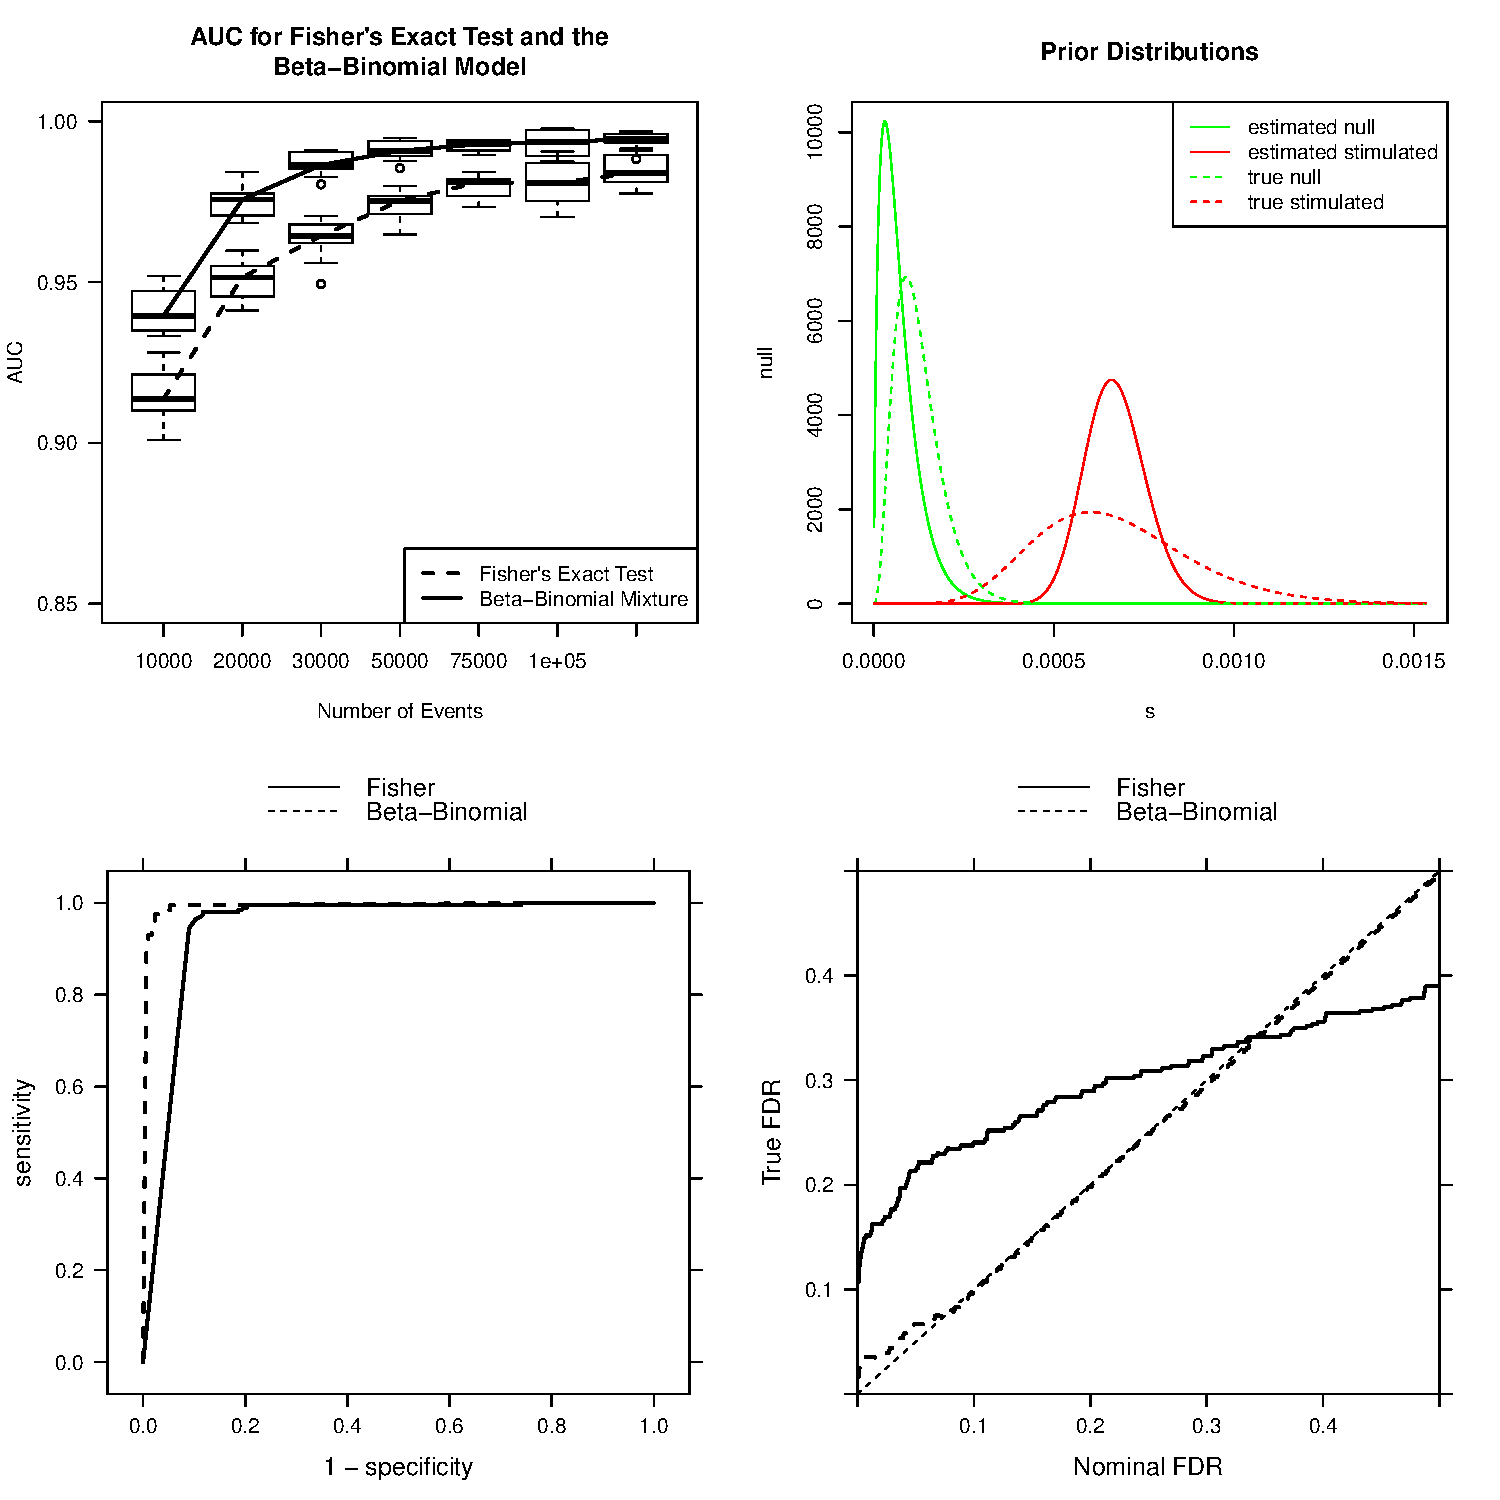
\includegraphics[width=4in]{Figures/simulations} 
   \caption{Performance of the constrained Beta-binomial mixture vs Fisher's exact test in simulated data from a constrained model. Data were simulated from a constrained model with hyper--parameters estimated from day 28, Gag1 stimulated, CD4+, IL2 expressing T--cells in the HVTN054 data set. We simulated 500 observations, with a response rate of 40\%, and increasing numbers of cells, ten times each. The performance, measured by the AUC, of the constrained beta--binomial mixture compared to Fisher's exact test is shown in the first panel, as a function of increasing number of events. The estimated and true prior distributions are shown in the second panel for one simulated data set, with N=150,000 events. The ROC curve for Fisher's exact test and the constrained Beta--binomial model for the same simulated data set are shown in the third panel. The observed vs expected false discovery rate for Fisher's exact test and the constrained Beta--binomial model are shown for the same data set in the fourth panel.}
   \label{fig:simulations}
\end{figure}

\begin{figure}[htbp] %  figure placement: here, top, bottom, or page
   \centering
   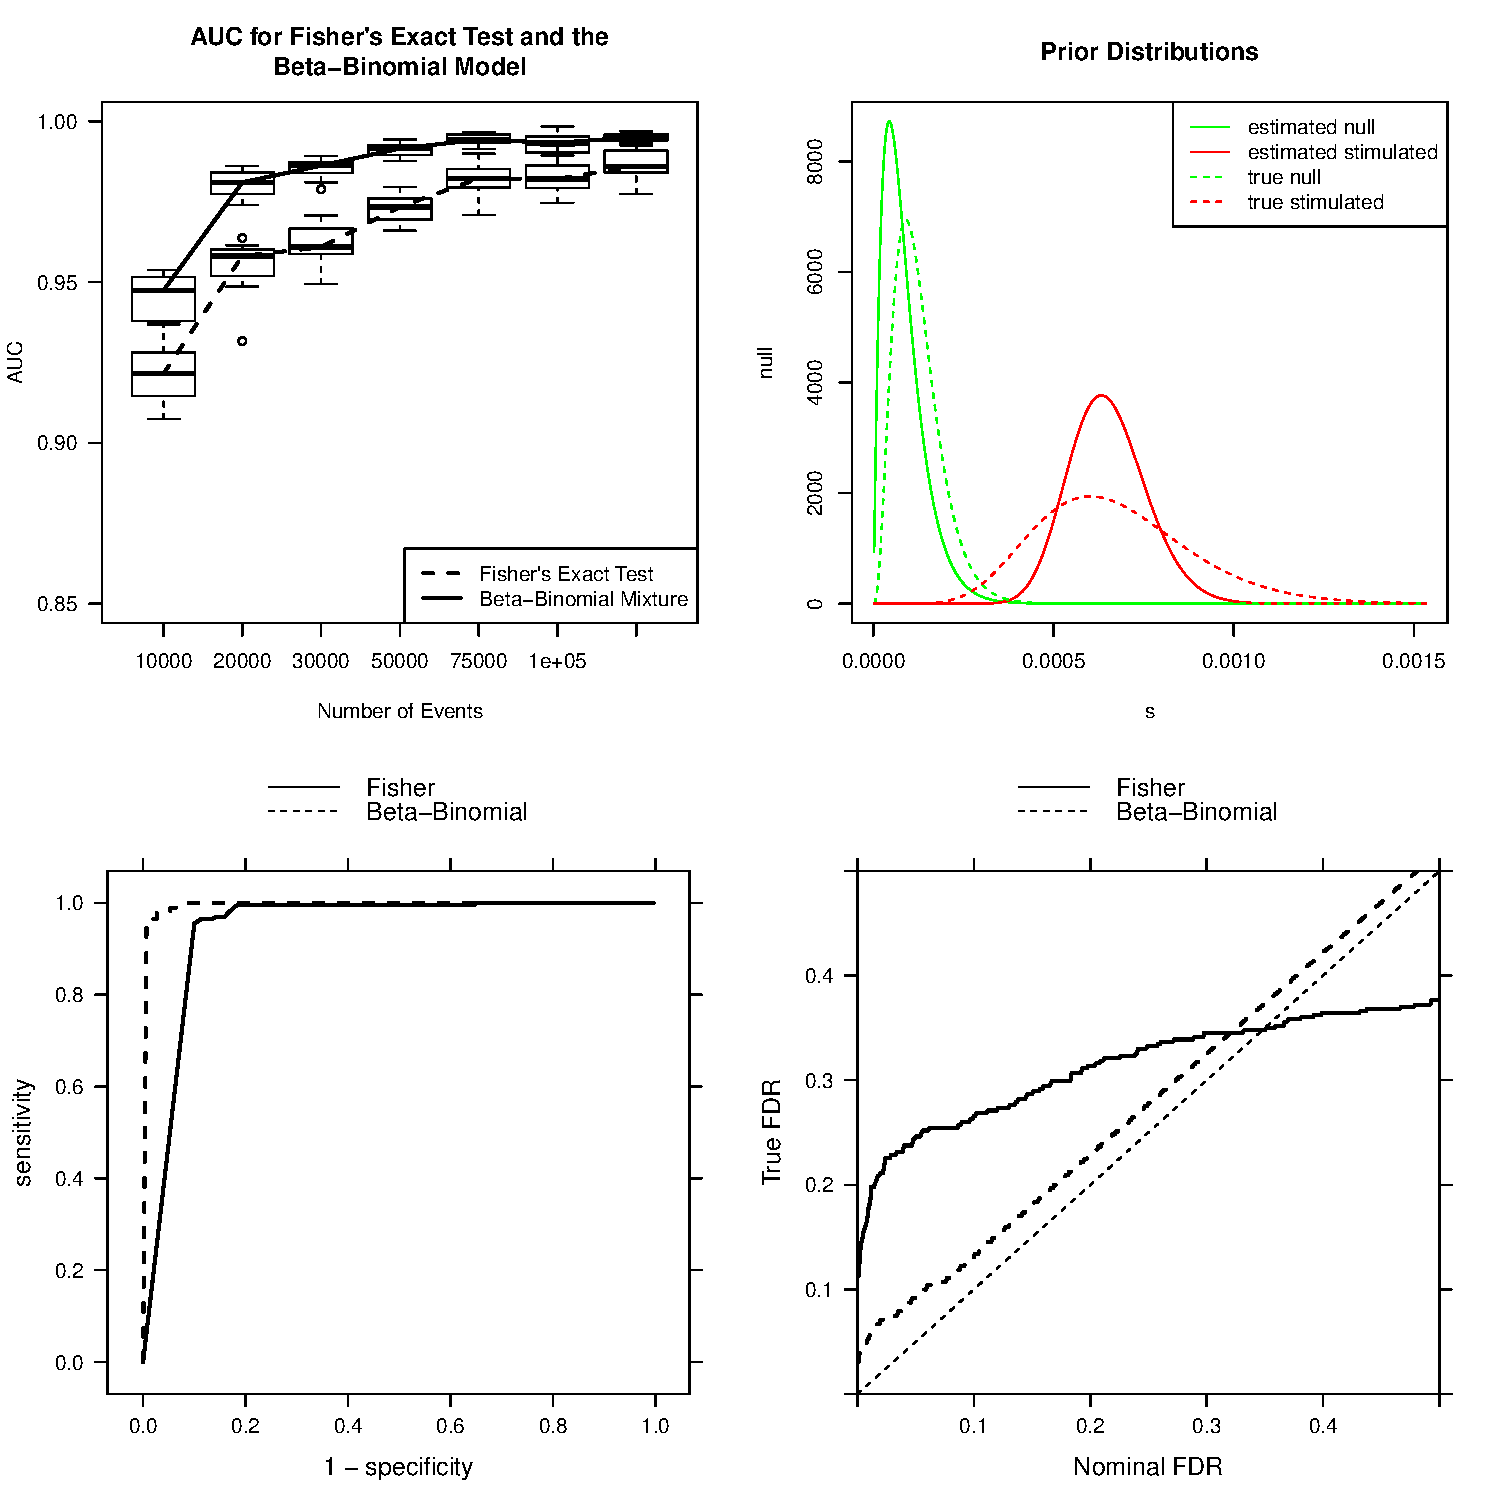
\includegraphics[width=4in]{Figures/simulations_negt} 
   \caption{Performance of the unconstrained Beta-binomial mixture (unconstrained model) vs Fisher's exact test in simulated data from a constrained model. Data were simulated from a constrained model with hyper--parameters estimated from day 28, Gag1 stimulated, CD4+, IL2 expressing T--cells in the HVTN054 data set. We simulated 500 observations, with a response rate of 40\%, and increasing numbers of cells, ten times each. The performance, measured by the AUC, of the unconstrained beta--binomial mixture compared to Fisher's exact test is shown in the first panel, as a function of increasing number of events. The estimated and true prior distributions are shown in the second panel for one simulated data set, with N=150,000 events. The ROC curve for Fisher's exact test and the unconstrained Beta--binomial model for the same simulated data set are shown in the third panel. The observed vs expected false discovery rate for Fisher's exact test and the Beta--binomial model are shown for the same data set in the fourth panel.}
   \label{fig:simulations}
\end{figure}

\subsection*{HVTN054 ICS Data}
\begin{figure}[htbp] %  figure placement: here, top, bottom, or page
   \centering
   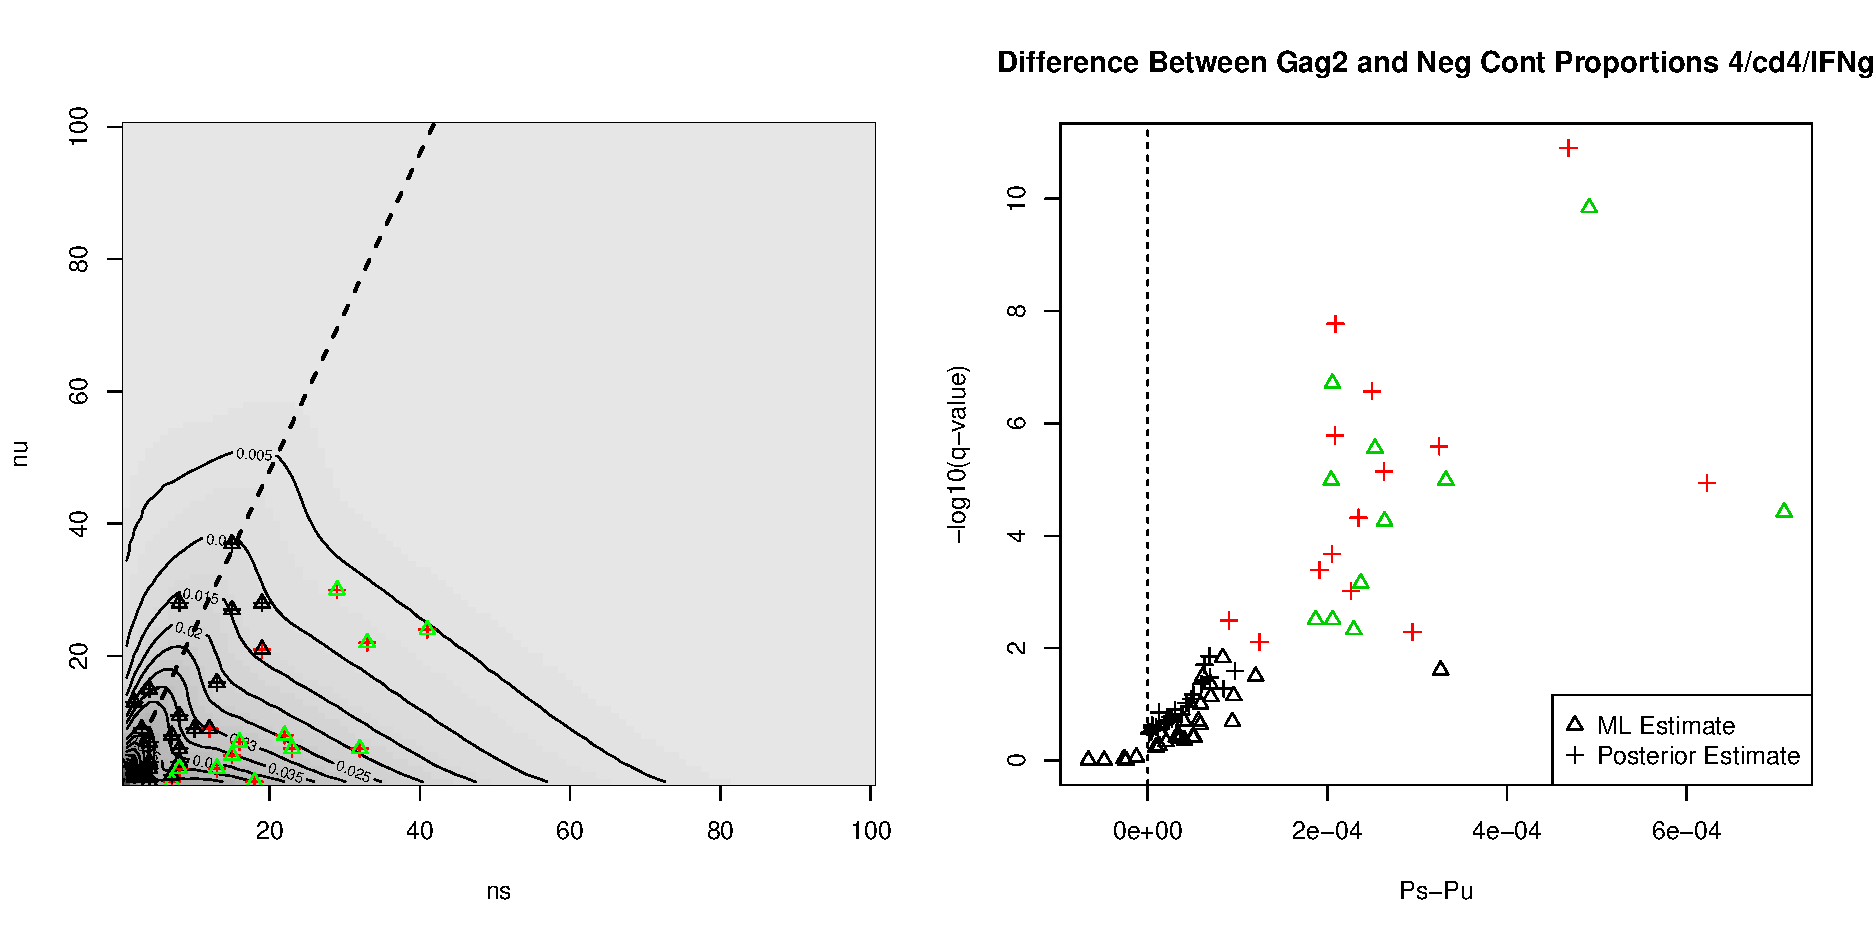
\includegraphics[width=6in]{Figures/HVTN054LikelihoodAndVolcanoplots} 
   \caption{Likelihood surface and volcano plot for IFNg producing, CD4+ T-cells in Gag2 stimulated vs control samples on day 28. A significant difference between control and stimulated samples is called at the 1\% FDR threshold (red) for the Beta--binomial model, and at 1\% for FDR adjusted p--values from Fisher's exact test (green). The likelihood surface shows the observed counts from stimulated and unstimulated samples. The volcano plot shows the difference between the proportion of cytokine positive cells in the stimulated and unstimulated samples, for the maximum likelihood estimates of the proportions (triangles) and for the MAP estimates (crosses)}
   \label{fig:simulations}
\end{figure}

\section*{Discussion}

\section*{Conclusions}

%\renewcommand{\thesection}{S.\arabic{section}}
%\renewcommand{\thesubsection}{\thesection.\arabic{subsection}}
%\todo[inline]{Note that the Supplementary Information section needs corrections to notation and overall}
%\section{Supplementary Information}
%\subsection{Derivation of the Beta--Binomial Model for $p_s=p_u$ and $p_s>p_u$}
%\label{sec:derivation}
%
%We derive the posterior predictive distribution and marginal log--likelihood for the null model ($p_s=p_u$) and the alternative model ($p_s>p_u$) below: patient indices, $i$ on the $\left<N_s,n_s,N_u,n_u\right>$ are omitted for clarity. 
%For model \eqref{eq:null}, ($p_s=p_u, \alpha_s=\alpha_u, \beta_s=\beta_u$), the posterior predictive distribution of the data given the model is:
% \begin{align}
% 	\mathrm{Pr}(y_i|\alpha_u,\beta_u) &= \int\limits_{p_u=0}\limits^{1} \mathrm{Pr}(y_i,p_u|\alpha_u,\beta_u)dp_u\\
%	&=\int\limits_{p_u=0}\limits^{1} \mathrm{Pr}(y_i|p_u)\mathrm{Pr}(p_u|\alpha_u,\beta_u)dp_u\\
%	\begin{split}
%		=\int\limits_{p_u=0}\limits^{1}\binom{N_s+n_s}{n_s}p_u^{n_s}(1-p_u)^{N_s}\binom{N_u+n_u}{n_u}p_u^{n_u}(1-p_u)^{N_u}\cdot \\ 
%		\frac{1}{\mathrm{B}(\alpha_u,\beta_u)}p_u^{\alpha_u-1}(1-p_u)^{\beta_u-1}dp_u
%	 \end{split}\\
%	 \begin{split}
% 	=\binom{N_s+n_s}{n_s}\binom{N_u+n_u}{n_u}\frac{1}{\mathrm{B}(\alpha_u,\beta_u)}\cdot\\ \int\limits_{p_u=0}\limits^{1}p_u^{n_s+n_u+\alpha_u-1}(1-p_u)^{N_s+N_u+\beta_u-1}dp_u
%	\end{split}\\
%	\intertext{The integrand is the kernel of a beta distribution with parameters $\left(n_u+n_s+\alpha_u,N_u+N_s+\beta_u\right)$, giving a closed form expression for the  posterior predictive distribution of model \eqref{eq:null}:}
%	\mathrm{Pr}(y_i|\alpha_u,\beta_u)&=\binom{N_s+n_s}{n_s}\binom{N_u+n_u}{n_u}\frac{\mathrm{B}(n_s+n_u+\alpha_u,N_s+N_u+\beta_u)}{\mathrm{B}(\alpha_u,\beta_u)}\label{eq:model1postsupp}\\
%	\intertext{with marginal log--likelihood:}
%	\begin{split}
%	\mathcal{L}(\alpha_u,\beta_u|\mathbf{y})=\sum_{i=1}^P\left[\log{\binom{N^i_{s}+n^i_{s}}{n^i_{s}}}+\log{\binom{N^i_{u}+n^i_{u}}{n^i_{u}}}+\right.\\
%	\left.\log{\left(\mathrm{B}(n^i_s+n^i_u+\alpha_u,N^i_s+N^i_u+\beta_u)\right)}\right]-P\log\left(\mathrm{B}(\alpha_u,\beta_u)\right)\label{eq:model1MLLsupp}
%	\end{split}
% \end{align} 
% 
%For model \eqref{eq:alternate}, ($p_s>p_u$), the posterior predictive distribution of the data given the model is:
%\begin{align}
% 	\mathrm{Pr}(y_i|\alpha_u,\beta_u,\alpha_s,\beta_s) &= \int\limits_{p_u=0}\limits^1\int\limits_{p_s>p_u}\limits^{1} \mathrm{Pr}(y_i,p_u,p_s|\alpha_u,\beta_u,\alpha_s,\beta_s) dp_u  dp_s\label{eq:postpredmodel2}\\
%	\intertext{Assuming independence of stimulated and unstimulated observations in \eqref{eq:postpredmodel2}:} 
%	&=\int\limits_{p_u=0}\limits^{1}\int\limits_{p_s>p_u}\limits^1 \mathrm{Pr}(n_s|p_s)\mathrm{Pr}(n_u|p_u)\mathrm{Pr}(p_u|\alpha_u,\beta_u)\mathrm{Pr}(p_s|\alpha_s,\beta_s)dp_u dp_s\\
%		&=\int\limits_{p_u=0}\limits^{1}\mathrm{Pr}(n_u|p_u)\mathrm{Pr}(p_u|\alpha_u,\beta_u)dp_u \int\limits_{p_s>p_u}\limits^1 \mathrm{Pr}(n_s|p_s)\mathrm{Pr}(p_s|\alpha_s,\beta_s)dp_s\\
%		\begin{split}
%	=\int\limits_{p_u=0}\limits^{1}\left[ \binom{N_u+n_u}{n_u}p_u^{n_u}(1-p_u)^{N_u} \frac{1}{\mathrm{B}(\alpha_u,\beta_u)}p_u^{\alpha_u-1}(1-p_u)^{\beta_u-1}d p_u\right]\cdot \\ \int\limits_{p_s>p_u}\limits^{1}\left[ \binom{N_s+n_s}{n_s}p_s^{n_s}(1-p_s)^{N_s} \frac{1}{\mathrm{B}(\alpha_s,\beta_s)}p_s^{\alpha_s-1}(1-p_s)^{\beta_s-1}d p_s\right]
%	\end{split}\\
%	\begin{split}
%	 =\binom{N_u+n_u}{n_u} \binom{N_s+n_s}{n_s}\frac{1}{\mathrm{B}(\alpha_u,\beta_u)}\frac{1}{\mathrm{B}(\alpha_s,\beta_s)}\cdot\\
%	 \int\limits_{p_u=0}\limits^{1}\left[p_u^{n_u+\alpha_u-1}(1-p_u)^{N_u+\beta_u-1} d p_u\right]\int\limits_{p_s>p_u}\limits^{1}\left[p_s^{n_s+\alpha_s-1}(1-p_s)^{N_s+\beta_s-1}d p_s\right]
%	\end{split}
%	\end{align}
%	\begin{align}
%	\begin{split}
%	 =\binom{N_u+n_u}{n_u} \binom{N_s+n_s}{n_s}\frac{1}{\mathrm{B}(\alpha_u,\beta_u)}\frac{1}{\mathrm{B}(\alpha_s,\beta_s)}\cdot\\
%	 \int\limits_{p_u=0}\limits^{1}\left[p_u^{n_u+\alpha_u-1}(1-p_u)^{N_u+\beta_u-1}d p_u \right]\left(1-\int\limits^{p_u}\limits_{p_s=0}\left[p_s^{n_s+\alpha_s-1}(1-p_s)^{N_s+\beta_s-1}d p_s\right]\right)
%	\end{split}
%	\intertext{The second integral can be expressed as the CDF of the beta distribution, also known as the regularized incomplete beta function, $\mathrm{I}_x(\alpha,\beta)$}
%	\begin{split}
%	 =\binom{N_u+n_u}{n_u} \binom{N_s+n_s}{n_s}\frac{1}{\mathrm{B}(\alpha_u,\beta_u)}\frac{\mathrm{B}(n_s+\alpha_s,N_s+\beta_s)}{\mathrm{B}(\alpha_s,\beta_s)}\cdot\\
%	 \int\limits_{p_u=0}\limits^{1}\left[p_u^{n_u+\alpha_u-1}(1-p_u)^{N_u+\beta_u-1} \right]\left(1-\mathrm{I_{p_s}}(n_s+\alpha_s,N_s+\beta_s)\right)d p_u
%	\end{split}\\
%	\intertext{giving the posterior predictive distribution of model \eqref{eq:alternate}}
%	\begin{split}
%		 =\binom{N_u+n_u}{n_u} \binom{N_s+n_s}{n_s}\frac{\mathrm{B}(n_u+\alpha_u,N_u+\beta_u)}{\mathrm{B}(\alpha_u,\beta_u)}\frac{\mathrm{B}(n_s+\alpha_s,N_s+\beta_s)}{\mathrm{B}(\alpha_s,\beta_s)}\cdot\\
%	 \int\limits_{p_u=0}\limits^{1}\left[\frac{1}{\mathrm{B}(n_u+\alpha_u,N_u+\beta_u)}p_u^{n_u+\alpha_u-1}(1-p_u)^{N_u+\beta_u-1} \right]\left(1-\mathrm{I_{p_u}}(n_s+\alpha_s,N_s+\beta_s)\right)d p_u\label{eq:model2postsupp}
%	\end{split}
%\end{align}
%The integral in equation~\eqref{eq:model2postsupp} is computed numerically. The marginal log--likelihood of model~\eqref{eq:alternate} is then:
%\begin{equation}
%		 \begin{split}
%		 \mathcal{L}(\alpha_s,\alpha_u,\beta_s,\beta_u|\mathbf{y})=-P\log\left(\mathrm{B}(\alpha_u,\beta_u)\right)-P\log\left(\mathrm{B}+(\alpha_s,\beta_s)\right)+\\ \sum_{i=0}^P\left\{\log\binom{N^i_u+n^i_u}{n^i_u}+ \log\binom{N^i_s+n^i_s}{n^i_s}+ \log\left(\mathrm{B}(n^i_u+\alpha_u,N^i_u+\beta_u)\right)+ \log\left(\mathrm{B}(n^i_s+\alpha_s,N^i_s+\beta_s)\right)+\right. \\ \left. \log\left(\hspace{1em}\int\limits_{p_u=0}\limits^{1}\left[\frac{1}{\mathrm{B}(n^i_u+\alpha_u,N^i_u+\beta_u)}p_u^{n^i_u+\alpha_u-1}(1-p_u)^{N^i_u+\beta_u-1} \right]\left(1-\mathrm{I_{p_u}}(n^i_s+\alpha_s,N^i_s+\beta_s)\right)d p_u\right)\right\}\label{eq:model2MLLsupp}
%\end{split}
%\end{equation}
%\subsection{The Beta-Binomial Mixture Model}
%For a given stimulation, not all individuals are expected to exhibit an immune response to that stimulation. Therefore, for a set of ICS data, any single observation, ($n^i_s,n^i_u$) could either be derived from model~\eqref{eq:null}, or from model~\eqref{eq:alternate}. We model this situation explicitly using a mixture--model framework.
\clearpage
\bibliographystyle{unsrtnat}
\bibliography{MIMOSA}

\end{document}  
